% !TEX encoding = UTF-8 Unicode
% LaTeX file for resume 
% This file uses the resume document class (res.cls)

\documentclass{res} 
\usepackage{fontspec}
\usepackage{xeCJK}
\usepackage{listings}
\usepackage[autostyle]{csquotes} 
\usepackage{hyperref}
\lstset{language=C,
numberstyle=\footnotesize,
basicstyle=\ttfamily\footnotesize,
numbers=left,
stepnumber=1,
frame=shadowbox,
breaklines=true}
\setCJKmainfont{STHeiti} % chinese type
%\setCJKmainfont{BiauKai}
%\usepackage{helvetica} % uses helvetica postscript font (download helvetica.sty)
%\usepackage{newcent}   % uses new century schoolbook postscript font 
\setlength{\textheight}{9.5in} % increase text height to fit on 1-page 
\usepackage{enumitem}

\XeTeXlinebreakskip = 0pt plus 1pt 

\begin{document} 


\name{\LARGE Real Time System Project1 Report}     % the \\[12pt] adds a blank
				        % line after name
\address{\\R03922106 蔡佑隆 unzledick@yahoo.com.tw\\ R04922067 楊翔雲 morris821028@gmail.com}

\begin{resume}

\vspace*{.1in} \noindent {\large \bfseries 作業描述}

安裝 linux kernel 2.6.32.68、練習 pthread 設定 scheduler 相關函數以利後續修改 kernel source code。

\vspace*{.1in} \noindent {\large \bfseries 安裝 Linux Kernel 步驟說明}

\begin{itemize}
	\item \lstinline{apt-get install fakeroot build-essential kernel-package libncurses5 libncurses5-dev}: 
	Ubuntu 安裝套件 \lstinline{fakeroot} 、 \lstinline{build-essential} 、 ... 等。
	
	\begin{itemize}
		\item \lstinline{fakeroot}: 模擬 root 權限執行指令,實際上並沒有 root 權限 (因遠端無法取得 root 權限)。
		\item \lstinline{build-essential}: 安裝 GNU Mach 需要 \lstinline{build-essential} package,包含 linux 開發的必要工具。
		\item \lstinline{libncurses libncurses5-dev}: 為 Linux 介面的圖形函數庫與開發工具。
	\end{itemize}
	
	\item \lstinline{sudo wget https://cdn.kernel.org/pub/linux/kernel/v2.6/lon gterm/v2.6.32/linux-2.6.32.68.tar.xz}: 從 Linux 官網下載 2.6.32.68 的 kernal 版本 (最新的版本為 4.x.x),用 root 權限安裝到 \lstinline{/usr/src} 中。
	
	\item \lstinline{make mrproper}: 刪除編譯過程中的目標檔案以及設定檔,連以前的 kernel 設定檔一起刪掉,原則上只有第一次執行核心編輯前才進行這個動作。
		\begin{itemize}
			\item \lstinline{make clean}: 不會刪除設定檔,僅編譯過程產生的中間檔案。
		\end{itemize}
	\item \lstinline{make menuconfig}: 在開機的圖形介面設定。重新啟動時,利用方向鍵選擇舊的 kernel 進行開機。
	
	\item \lstinline{make bzImage}: 編譯 kernel 且這個 kernel 是經過壓縮,步驟也很長。
	
	\item \lstinline{make module}: 將上一個步驟產出的模組,進行編譯,速度取決於 \lstinline{make bzImage}
	
	\item \lstinline{make modules_install}: 安裝 modules,如安裝版本 2.6.32.68,模組檔案會產生於 \lstinline{/lib/modules/2.6.32.68}。
	
	\item \lstinline{make install}: 安裝 \lstinline{bzImage} 建立好的模組。
	
	\item  \lstinline{#GRUB_HIDDEN_TIMEOUT=10, #GRUB_HIDDEN_TIMEOUT_QUIET=true}: 強迫顯示出 grub 選單,進入舊的 kernel 使用。
	
	\item \lstinline{update-grub2}: 將 grub 更改的內容更新至 grub.cfg (GBUB2 利用它來設定進入 BIOS)
\end{itemize}

\vspace*{.1in} \noindent {\large \bfseries 實驗討論}

\hspace*{.1in} \noindent {\bfseries 設定 scheduler 問題}

\begin{itemize}
	\item 設定 thread 可以在哪些 core 運行,由於要測試執行順序,強制讓 pthread 都在 CPU 0 運行。編譯時,增加 \lstinline{#define _GNU_SOURCE} 在 \lstinline{#include <pthread>} 之前,確定 \lstinline{cpu_set_t} 型別存在。
	
\begin{lstlisting}[frame=single]
cpu_set_t mask;
CPU_ZERO(&mask);
CPU_SET(0, &mask);
sched_setaffinity(0, sizeof(mask), &mask);
\end{lstlisting}

	\item 使用 \lstinline{sched_setscheduler()} 時,需查閱 \lstinline{int policy} 相關規定去設定 \lstinline{struct sched_param} 的 priority 數值。例如 \lstinline{SCHED_FIFO} 的 priority 介於 1 到 99 之間,若 priority 錯誤,\lstinline{sched_setscheduler()} 會發生錯誤,錯誤訊息可以藉由 \lstinline{printf("Message %s\n", mid, strerror(errno));} 查閱。

\begin{lstlisting}[frame=single]
int sched_setscheduler(pid_t pid, int policy,
                              const struct sched_param *param);
\end{lstlisting}

如果 pid = 0,相當於 caller 的 thread 會被設置對應的 \lstinline{policy} 和 \lstinline{sched_param}。在 policy 設定規範中,有兩種 real time scheduler \lstinline{SCHED_FIFO} 和 \lstinline{SCHED_RR}。當 thread 設置 real time scheduler 時,需要用 root 權限來執行程式,否則會設置失敗。相反地,若使用 non-real time scheduler 則不需要 root 權限,如 \lstinline{SCHED_BATCH}。

\begin{lstlisting}[frame=single]
struct sched_param param;
printf("Thread %d sched_setscheduler()\n", mid);
param.sched_priority = sched_get_priority_max(SCHED_FIFO);
s = sched_setscheduler(0, SCHED_FIFO, &param);
printf("Thread %d sched after %s\n", mid, strerror(errno));
\end{lstlisting}

\end{itemize}

\hspace*{.1in} \noindent {\bfseries 三種方法設定 pthread}

\begin{itemize}
	\item 各自的 \lstinline{pthread_create()} 後,再呼叫 \lstinline{sched_setscheduler()} 進行設定。這種寫法在本次實驗有順序問題,在 create 之後,無法保證執行 \lstinline{sched_setscheduler()} 的順序,無法依靠 main thread 中執行 \lstinline{pthread_create()} 的順序決定。幸運地,仍可以使用 
	
\begin{lstlisting}
pthread_barrier_t barrier; 
pthread_barrier_wait(&barrier);
pthread_barrier_init(&barrier, NULL, MAX_THREAD);
\end{lstlisting}

確保每一個 thread 都設置好各自的 \lstinline{sched_setscheduler()} 後統一運行,運行順序取決 priority。

	\item 在 main thread 中,呼叫 \lstinline{pthread_attr_setinheritsched(attr, PTHREAD_INHERIT_SCHED);} 接下來 create 出來的 pthread 都將繼承 main thread 的 scheduler 設定。這種寫法很方便,如果需要各自設置 priority 會不方便,倒不如直接用第三種寫法。
	
	\item 在 main thread 中,手動設置每一個 pthread 的 scheduler。
	
\begin{lstlisting}[frame=single]
pthread_attr_t *attr = new pthread_attr_t;
struct sched_param *param = new struct sched_param;
// increasing order
param->sched_priority = sched_get_priority_max(SCHED_FIFO) - i;
// set scheduler
pthread_attr_setinheritsched(attr, PTHREAD_EXPLICIT_SCHED);
pthread_attr_setschedpolicy(attr, SCHED_FIFO);
pthread_attr_setschedparam(attr, param);
// create thread
pthread_create(&tid[i], attr, running_print, create_arg(i+1, scheduler))
\end{lstlisting}

\end{itemize}

\hspace*{.1in} \noindent {\bfseries 計時設置}

\begin{itemize}
	\item 為確定每一個 thread 按照設定的 scheduler 運行,方式採用 \lstinline{print()} 進行,但有可能輸出之間間隔距離過短,導致順序容易在輸出上發生無法預期的問題,適時地加入一秒間隔完成。
	
	\item 如何準確地停止一秒?不能呼叫 \lstinline{sleep()} 因為這類的 system call 會產生 interrupt,此時 thread 將會降低 priority 或者進入隊列尾端。佔據 CPU time 有以下三種
	\begin{itemize}
		\item 只要停留的夠久即可,下面是一種簡單的方法	
\begin{lstlisting}
// busy 1 second
double a = 0;
for (int i = 0; i < 10000000; i++)	a += 0.1f;
\end{lstlisting}
		\item 利用 critical section 抓系統時間 \lstinline{int gettimeofday (struct timeval * tv, struct timezone * tz);},這寫法會共用同一份時間,因此需要使用 mutex 完成。仍使用一個迴圈來判定時間是否超過,實際運行時間會超過一秒。
\begin{lstlisting}[frame=single]
static double my_clock(void) {
	struct timeval t;
	gettimeofday(&t, NULL);
	return 1e-6 * t.tv_usec + t.tv_sec;
}
pthread_mutex_lock(&outputlock);
{
	double sttime = my_clock();
	while (1) {
		if (my_clock() - sttime > 1)
			break;
	}
}
pthread_mutex_unlock(&outputlock);
\end{lstlisting}

		\item 事實上 Linux 有提供每一個 thread 各自的 clock,用來計算 thread 的執行時間。使用 \lstinline{clock_gettime(CLOCK_THREAD_CPUTIME_ID, &t)},在舊版本需在編譯參數中加入 \lstinline{-lrt} 才能使用。
\begin{lstlisting}[frame=single]
static double my_clock(void) {
	struct timespec t;
	assert(clock_gettime(CLOCK_THREAD_CPUTIME_ID, &t) == 0);
	return 1e-9 * t.tv_nsec + t.tv_sec;
}
\end{lstlisting}

	\end{itemize}
\end{itemize}

\vspace*{.1in} \noindent {\large \bfseries 輸出 \lstinline{console} 問題}

\begin{itemize}
	\item 在 \lstinline{SCHED_FIFO} 這類的 real time scheduler 情況下,thread 輸出無法即時顯示在 terminal 上。
	
	\item 從 \url{http://man7.org/linux/man-pages/man7/sched.7.html} 可以見到 real-time scheduler 安排工作的比例,由於 \lstinline{print()} 之後的顯示處理並不是 real-time process,當 real-time process 完全用盡 95\% 的 CPU time 時,顯示處理可能沒辦法在一秒內完成,可能要用好幾秒中的 5\% 來完成。這也就是造成一開始會停頓一陣子,隨後才一次輸出數行結果。(註:並不是每一種裝置都會造成這問題,跟 CPU 時脈有關。)
	\blockquote{The value in this file specifies how much of the period time  can be used by all real-time and deadline scheduled processes on the system.  The value in this file can range from \lstinline{-1} to \lstinline{INT_MAX-1}.  Specifying \lstinline{-1} makes the runtime the same as the period; that is, no CPU time is set aside for non-real-time processes (which was the Linux behavior before kernel 2.6.25). The default value in this file is 950,000 (0.95 seconds), meaning that 5\% of the CPU time is reserved for processes that don't run under a real-time or deadline scheduling policy.}
	
	\item 解決這類的問題,可以從 kernel 設定著手,降低 real-time 最大佔有量,讓 \lstinline{print()} 處理能即刻印出。這不是好的解決辦法,但可用於實驗。
\begin{lstlisting}
// default
$ sudo /sbin/sysctl -w kernel.sched_rt_runtime_us=950000
// modify
$ sudo /sbin/sysctl -w kernel.sched_rt_runtime_us=500000
\end{lstlisting}

	\item 又或者採用拉大間隔,讓每一個 thread 都停止數十秒以上。
	\item 特別感謝:蕭光宏學長
\end{itemize}

\vspace*{.1in} \noindent {\large \bfseries 執行結果}

\begin{figure}[htp]
    \begin{center}
        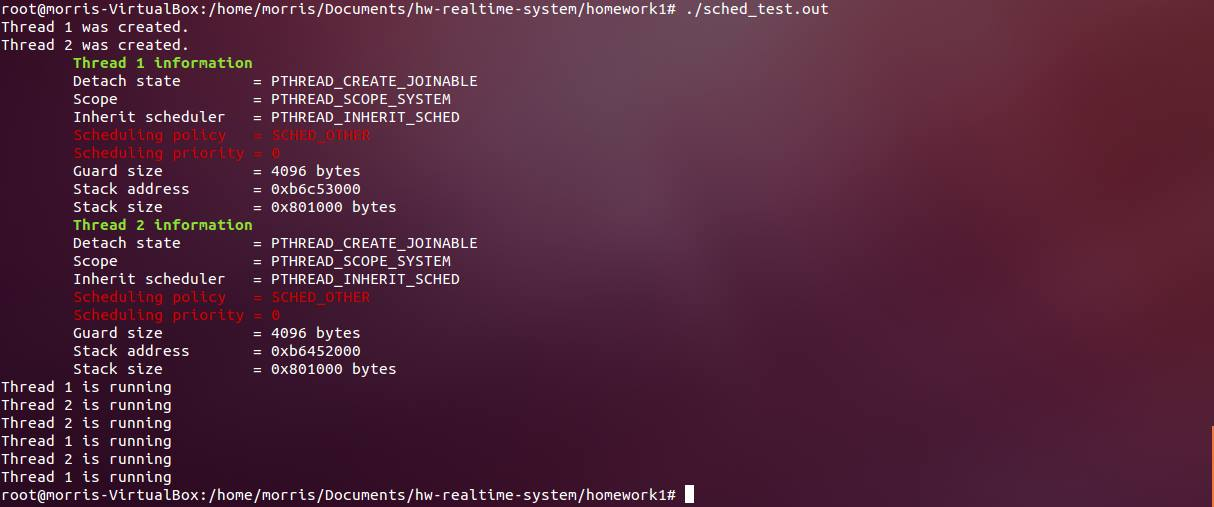
\includegraphics[width=400pt]{images/result1.jpg}
        \caption{Default Scheduler 執行結果}
        \label{fig: result}
    \end{center}
\end{figure}

\begin{figure}[htp]
    \begin{center}
        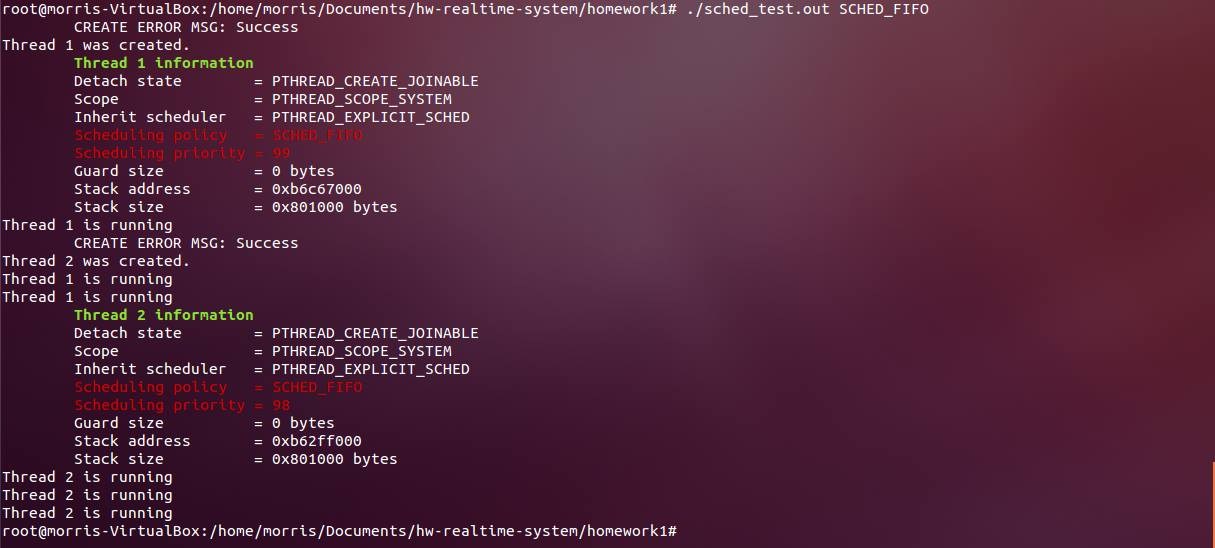
\includegraphics[width=400pt]{images/result2.jpg}
        \caption{FIFO Scheduler 執行結果}
        \label{fig: result}
    \end{center}
\end{figure}

\end{resume}



\end{document}